\chapter{Conclusions}

\section{Comparison of Training and Prediction Times}

It can be seen from the below charts that there are substantial differences between certain types of classifiers, both when considering training and prediction times.
It is noted that time have been normalized so that the highest value is equal to one, to make the charts somewhat platform-independent.

\paragraph{Training Time} The models that took the longest time to train were the SVMs. This has to do with what was highlighted at \ref{svm_kernel_trick_and_complexity} about the asymptotic complexity of the training phase. Additionally, as regards to the other classifiers, which took far less time to train:

\begin{itemize}
    \item Random Forest benefitted from a high level of parallelization
    \item the complexity of the Naive Bayes one is close to linear
    \item KNN is a lazy model that doesn't do any calculation in the training phase
\end{itemize}

\paragraph{Prediction Times} From the prediction times chart, one model is outstanding: Naive Bayes. This has to do with the implementation, which didn't make enough use of vectorization and the \textit{numpy} library, which would have probably improved times by a factor of at least 10. If it wasn't for this outlier, the longest times to predict 10k samples would be those of the SVM and KNN models, due to both having quadratic time complexity. The RandomForestClassifier is the best performing one, possibly, again, due to it being extremely well suited for parallelization.

\begin{figure}[h]
    \centering

    \begin{minipage}{0.475\textwidth}   
        \centering 
        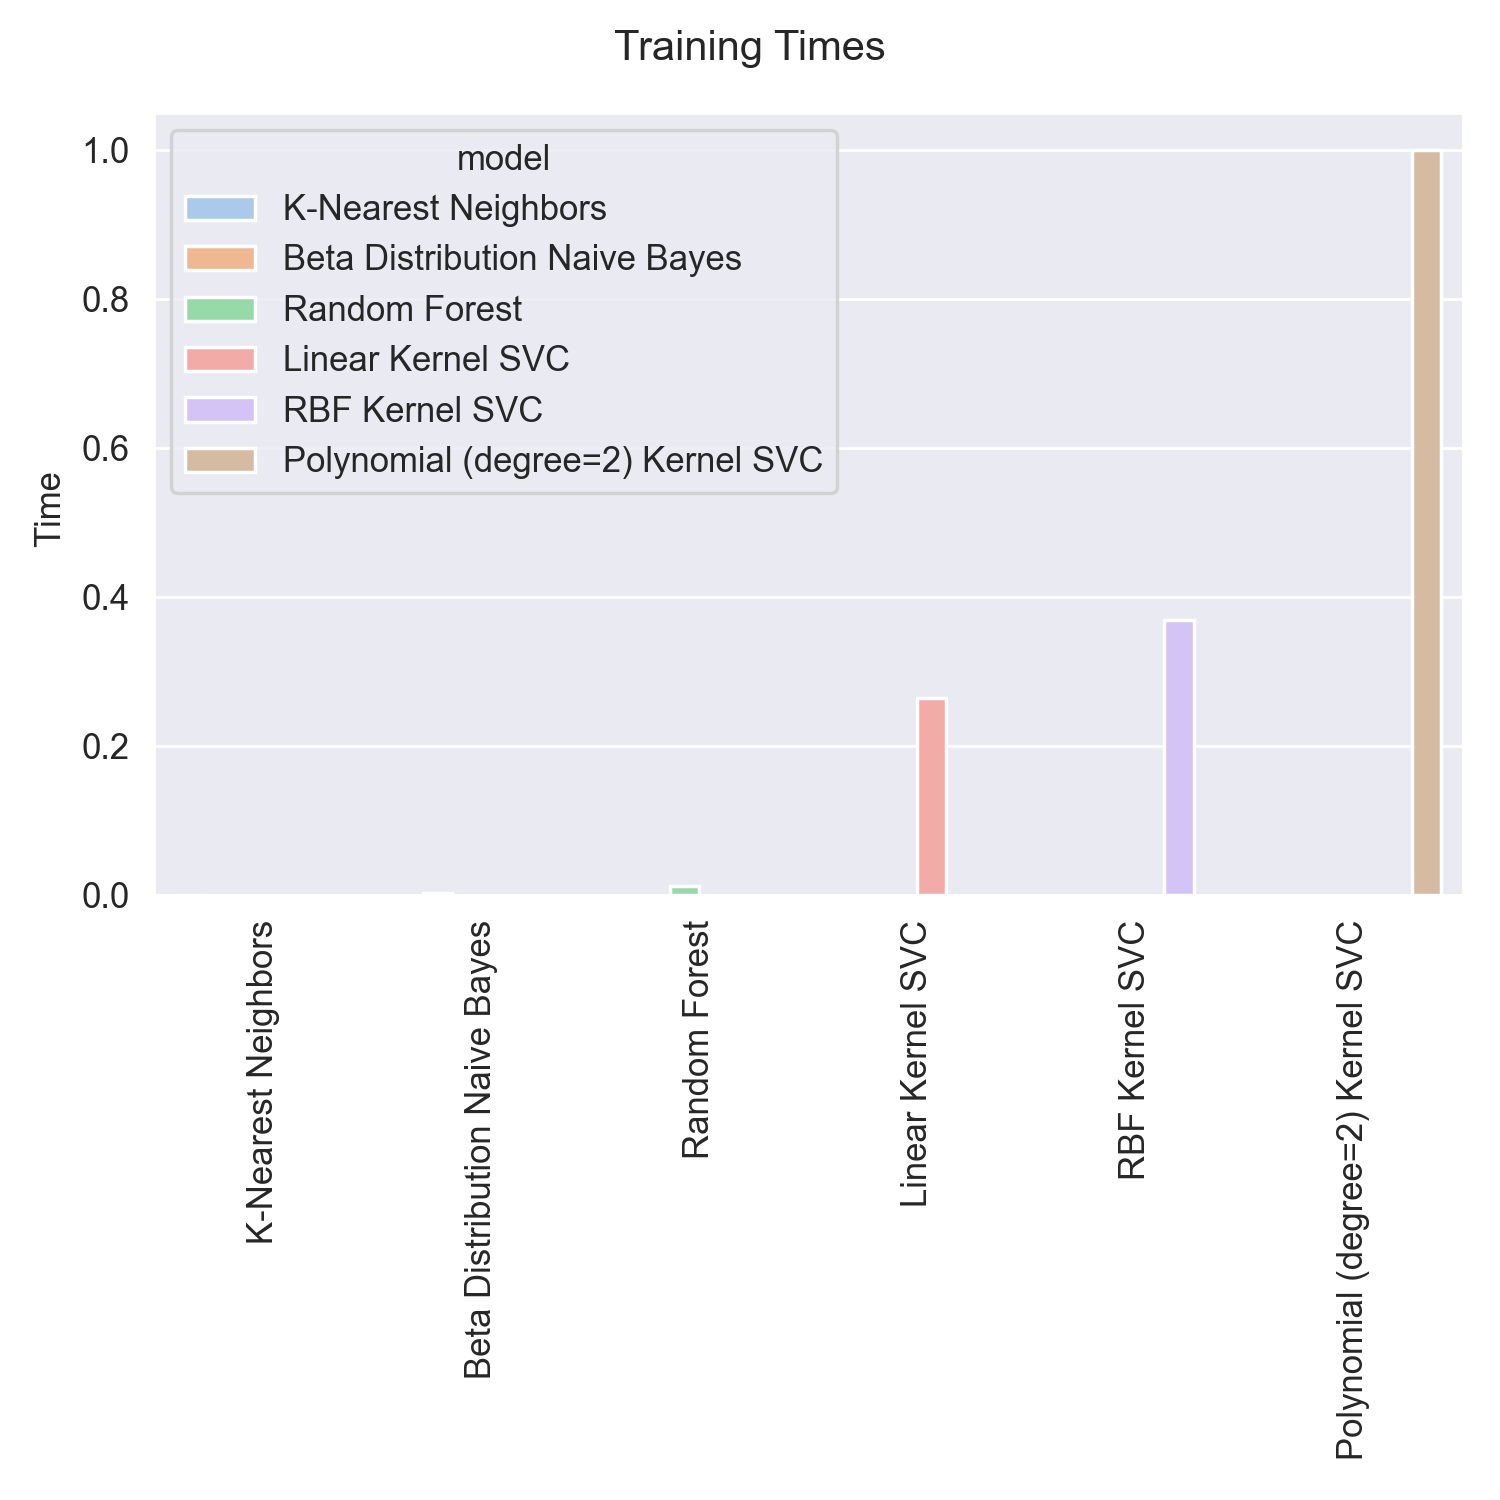
\includegraphics[scale=0.55]{images/exp-results/training_times.png}
        \label{fig:exp_res_training_time_all}
        % \caption{Training time of each classifier on the full training set (normalized)}
    \end{minipage}
    \hspace{.025\linewidth}
    \begin{minipage}{0.475\textwidth}
        \centering
        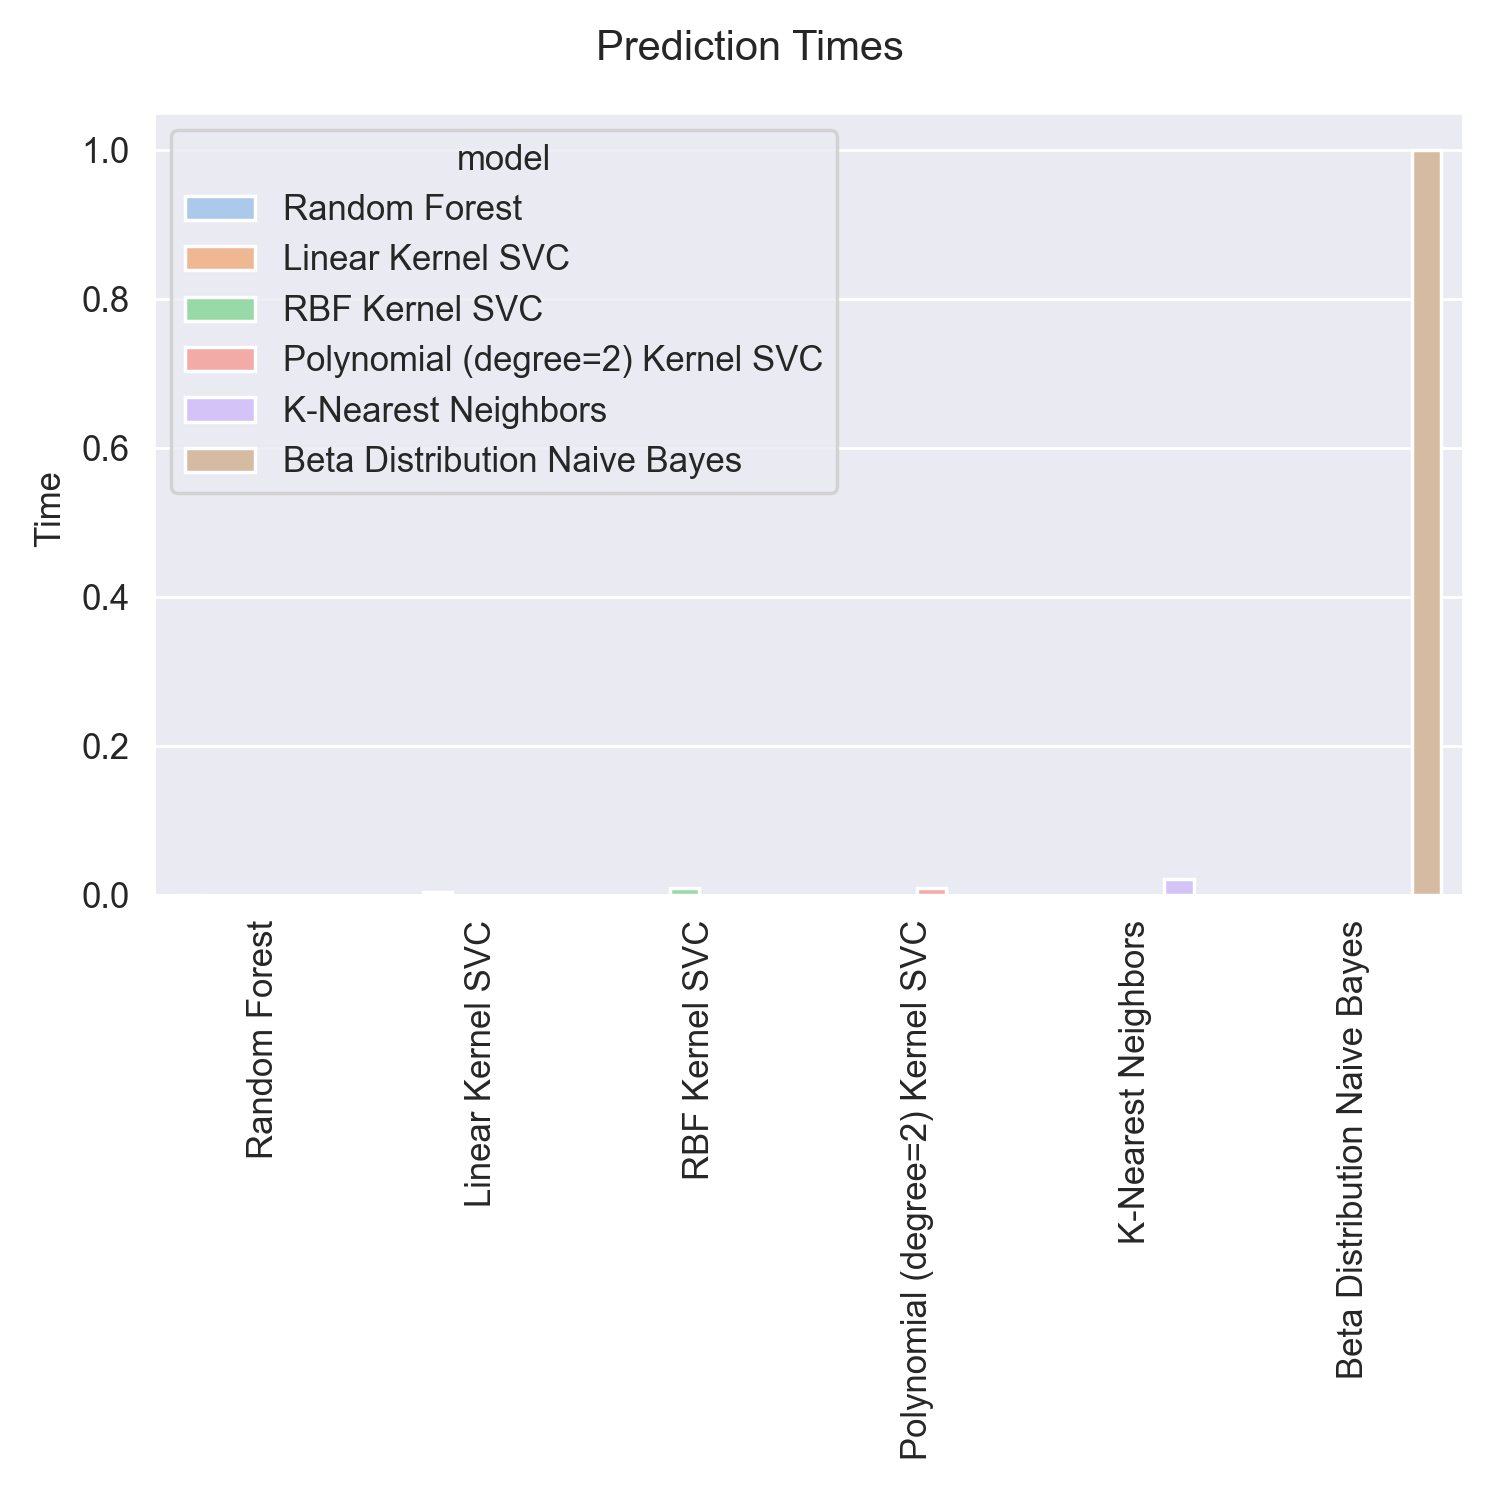
\includegraphics[scale=0.55]{images/exp-results/prediction_times.png}
        \label{fig:exp_res_pred_time_all}
        % \caption{Prediction time of each classifier on the testing set (normalized)}
    \end{minipage}
\end{figure}

\begin{figure}[h]
\end{figure}

\break
\section{Classification Performance: Generative vs Discriminative Classifiers}

\begin{figure}[h]
    \centering
    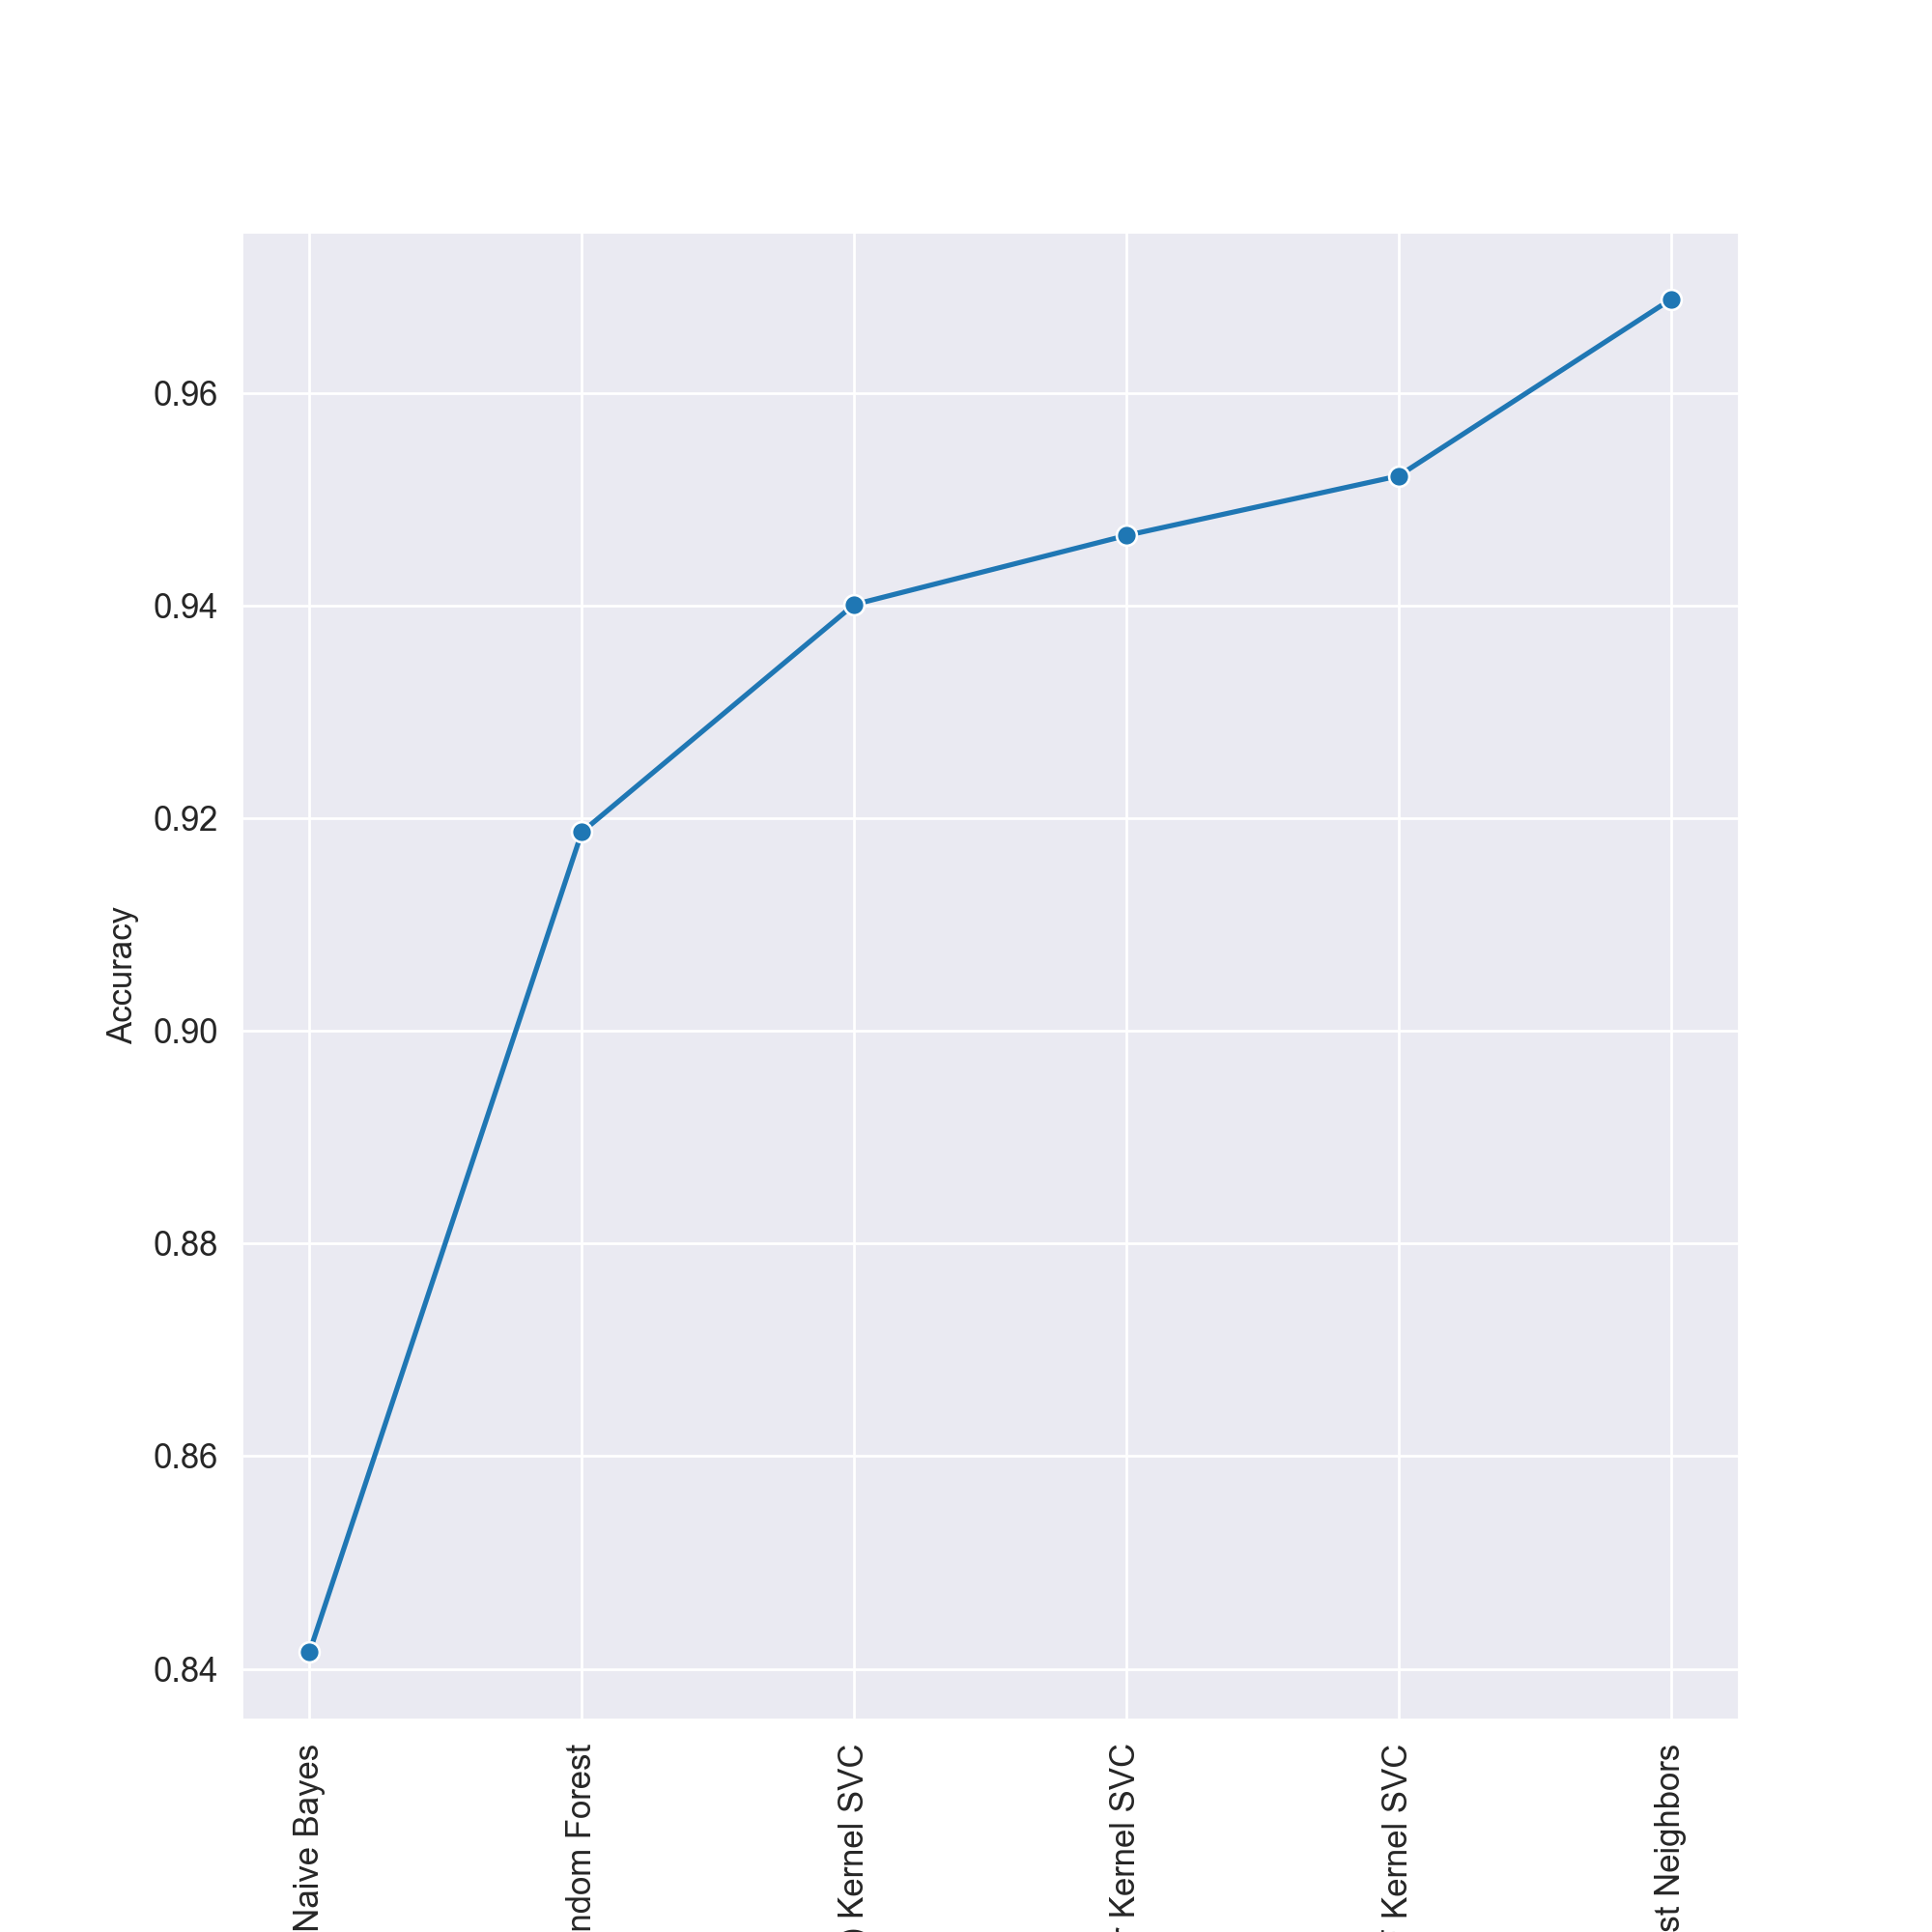
\includegraphics[scale=0.6]{images/exp-results/test_accuracy.png}
    \caption{Accuracy of each classifier on the testing set}
    \label{fig:exp_res_test_accuracy_all}
\end{figure}


As it could also be deduced from the results presented in chapter \ref{exp_results_chapter}, the classification task was on average more difficult when it involved digits from 2 to 9: this is because the distinguishing characteristics of such digits are similar and there is some overlap. For example, a \textit{3 is almost an 8 or a 5}, or a \textit{4 is almost a 9}.

This consideration also helps to explain why there was a strong difference in accuracy between discriminative and generative classifiers: the Beta Distribution Naive Bayes performed far worse than all the others. This might be because the feature distributions of similar digits are also quite similar, leading to misclassification. 
It is noted that such a problem is exacerbated by the fact that generative classifiers, by definition, do not try to find the best way to \textit{distinguish} different data points, while discriminative classifiers do, which may explain their more robust performance on this dataset.